\documentclass[xcolor=table]{beamer}
\usepackage{beamerthemesplit}
\usepackage{wrapfig}
\usetheme{SPbGU}
\usepackage{pdfpages}
\usepackage{amsmath}
\usepackage{amssymb}
\usepackage{cmap}
\usepackage[T2A]{fontenc}
\usepackage[utf8]{inputenc}
\usepackage[english]{babel}
\usepackage{indentfirst}
\usepackage{amsmath}
\usepackage{tikz}
\usepackage{multirow}
\usepackage[noend]{algpseudocode}
\usepackage{algorithm}
\usepackage{algorithmicx}
\usepackage{fancyvrb}
\usetikzlibrary{shapes,arrows}
\usepackage{tikz}
\usetikzlibrary{automata,positioning}
\usepackage[linguistics]{forest}
\usepackage{listings}
\usepackage{multicol}
\usepackage{comment}
\usepackage{ stmaryrd }
\usepackage{cancel}
\usepackage{hyperref}

\setbeamertemplate{itemize items}[circle]
\setbeamertemplate{enumerate items}[circle]

\lstset{
language=Haskell
}


\beamertemplatenavigationsymbolsempty

\title[]{A Framework for Building Verified Partial Evaluators\\~\\Построение сертифицированных частичных вычислителей}
\institute[]{
Лаборатория языковых инструментов JetBrains
}

\author[Екатерина Вербицкая]{Екатерина Вербицкая}

\date{20.04.2020}

\definecolor{orange}{RGB}{179,36,31}

\begin{document}
{
\begin{frame}[fragile]
   \begin{center}
      
\includegraphics[height=1.5cm]{pictures/jetbrainsResearch.pdf}
    \end{center}
  \titlepage
\end{frame}
}

\begin{frame}[fragile]
  \transwipe[direction=90]
  \frametitle{Частичные вычисления (partial evaluation)}
\[p(s,d)\]

\[peval(p, s) = p'\]

\[\forall d: \llbracket p'\rrbracket (d) \equiv \llbracket p \rrbracket (s, d) \]
\end{frame}

\begin{frame}[fragile]
  \transwipe[direction=90]
  \frametitle{Пример: двоичное возведение в степень}

\begin{lstlisting}
pow (n, a) = if n == 0
             then 1
             else if n `mod` 2 == 1
                  then pow (n - 1, a) * a
                  else let r = pow (n `div` 2, a)
                       in  r * r
\end{lstlisting}

\begin{lstlisting}
peval (pow, 10) = \ a -> ((a ^ 2) ^ 2 * a) ^ 2
\end{lstlisting}

\end{frame}

\begin{frame}[fragile]
  \transwipe[direction=90]
  \frametitle{Пример: префикс-суммы}
\[
  sum(lst, l) = \sum_{i=0}^{l} (i * lst[i])
\]

\[
  prefixSum(lst) = reverse \ lst', \text{ где } lst'[i] \equiv sum(lst, i)
\]

\bigskip

\begin{center}
  Хочется, чтобы в результате специализации получалось следующее:
\end{center}

\bigskip

\begin{lstlisting}
prefixSum ([a,b,c,d]) =
  let acc = b + c * 2 in
  let acc' = acc + d * 3 in
  [acc', acc, b, 0]
\end{lstlisting}

\end{frame}

\begin{frame}[fragile]
  \transwipe[direction=90]
  \frametitle{Зачем нужны частичные вычисления?}
\begin{center}
  Для улучшения производительности реализаций
\end{center}
\begin{itemize}
  \item Можно писать обобщенные библиотеки, потом специализировать под разные условия
  \item Улучшать в соответствии с правилами, верными в конкретном домене
  \item Не надо создавать свой компилятор, который знает про эти правила
\end{itemize}
\end{frame}


\begin{frame}[fragile]
  \transwipe[direction=90]
  \frametitle{Цели и контекст этой работы}
\begin{itemize}
  \item Улучшать существующие библиотеки, не адаптируя их
  \item Использование в сертифицированных системах
  \begin{itemize}
    \item Библиотеки реализованы на функциональном подмножестве Coq
    \item Частичные вычисления должны производиться \emph{быстро} и генерировать \emph{пруф-термы}, гарантирующие их корректность
    \item Количество доверенных компонент не должно увеличиться (нельзя добавлять новые стратегии редукций в ядро Coq)
  \end{itemize}
\end{itemize}
\end{frame}


\begin{frame}[fragile]
  \transwipe[direction=90]
  \frametitle{Вклад этой работы}
\begin{itemize}
  \item Фреймворк для создания сертифицированных частичных вычислителей
  \begin{itemize}
    \item Без изменений в Coq
    \item Высокая скорость частичных вычислений
    \item Использование для частичных вычисления definitional equality и пользовательских теорем
    \item Переиспользование общих подтермов
    \item Извлечение частичных вычислителей
    \item Поддержка правил переписывания с дополнительными условиями
  \end{itemize}
  \item Эвалюация на Coq библиотеке для криптографии Fiat Cryptography
\end{itemize}

Поддерживаются:

\begin{itemize}
  \item Функции высших порядков
  \item Индуктивные типы данных
  \item Арифметические законы
\end{itemize}
\end{frame}


\begin{frame}[fragile]
  \transwipe[direction=90]
  \frametitle{Пример про префикс-суммы}

\begin{center}
  код
\end{center}
\end{frame}

\begin{frame}[fragile]
  \transwipe[direction=90]
  \frametitle{Про доверенный код}
\begin{itemize}
  \item Важно не добавлять в ядро кода, которому доверяем
  \item Новые стратегии редукций могут быть полезны для производительности
  \item Невозможно обосновывать каждый маленький шажок преобразований
  \item Coq не требует обосновывать то, что следует из definitional equality
\end{itemize}

\bigskip
Решение: максимально использовать встроенный механизм редукций Coq
\end{frame}

\begin{frame}[fragile]
  \transwipe[direction=90]
  \frametitle{Подходы к переписыванию термов: definitional equality}

\begin{center}
    Основной механизм переписывания в Coq
\end{center}

\begin{itemize}
  \item $\beta$-редукция
  \item Замена идентификаторов на их значения
  \item Сопоставление с шаблоном при известном значении сопоставляемого
  \item $\dots$
\end{itemize}


\begin{center}
  Свободные переменные быстро водят в тупик
\end{center}
\end{frame}

\begin{frame}[fragile]
  \transwipe[direction=90]
  \frametitle{Подходы к переписыванию термов: autorewrite}
\begin{itemize}
  \item Используется база квантифицированных равенств
  \item Каждое равенство порождает фрагменты пруф-термов
  \bigskip
  \item В итоге получается много больших пруфтермов
  \begin{itemize}
    \item Для обоснования $C[e_1] = C[e_2]$, при условии $e_1 = e_2$ необходимо скопировать весь контекст $C$
  \end{itemize}
\end{itemize}
\end{frame}

\begin{frame}[fragile]
  \transwipe[direction=90]
  \frametitle{Подходы к переписыванию термов: Aehlig et al.}
\begin{center}
  Комбинирование вычислений над $\lambda$-термами и использования обоснованных равенств
\end{center}

\begin{itemize}
  \item На языке пруф-асистанта реализуется deep-embedded ML и его операционная семантика
  \item Для конкретного терма и правила переписывания порождается deep-embedded терм на ML, который будет порождать упрощенный терм (если завершается)
  \bigskip
  \item Много нового кода, которому нельзя доверять
  \item Нет гарантии, что семантика реализованного ML совпадает с тем, на котором будет исполняться частичные вычисления
\end{itemize}
\end{frame}

\begin{frame}[fragile]
  \transwipe[direction=90]
  \frametitle{Подходы к переписыванию термов: эта работа}
  \begin{itemize}
    \item Реализуем правила переписывания непосредственно на Coq, не на встроенном языке
    \item Используем ядро Coq для непосредственного осуществления редукций
  \end{itemize}
\end{frame}

\begin{frame}[fragile]
  \transwipe[direction=90]
  \frametitle{Создадание частичного вычислителя по шагам}
  \begin{itemize}
    \item Пользователь пишет леммы, которые будут использоваться для переписывания
    \item Порождаются индуктивные типы для всех примитивных типов и функций
    \item Порождаются вспомогательные определения и доказываются леммы, необходимые для работы с индуктивными определениями
    \item Реифицируются утверждения о правилах переписывания. Пользователь доказывает их полноту (soundness) и синтаксическую корректность (syntactic well-formedness)
    \item Все нужные утверждения передаются специальной тактике
  \end{itemize}
\end{frame}

\begin{frame}[fragile]
  \transwipe[direction=90]
  \frametitle{Применение частичного вычислителя}
  \begin{itemize}
    \item Цель превращается в логическую формулу
    \begin{itemize}
      \item Если в ней есть свободные переменные, то она превращается в функцию на этих переменных
    \end{itemize}
    \item Реифицируем часть, которую хотим упрощать
    \begin{itemize}
      \item Потом она заменяется на денотацию реифицированной версии
    \end{itemize}
    \item Используем теорему о том, что правило переписывания сохраняет денотацию термов, чтобы обосновать переписывание
    \begin{itemize}
      \item Для применения правила переписывания применяется vm-compute
    \end{itemize}
    \item Используем cbv для упрощения вызовов к денотации функции
  \end{itemize}
\end{frame}

\begin{frame}[fragile]
  \transwipe[direction=90]
  \frametitle{Выбор правила переписывания из набора}

\[?n + 0 \rightarrow n\]


\begin{center}
  \verb!App (App (Ident +) Wildcard) (Ident 0)!
\end{center}

\smallskip

\[fst_{\mathbb{Z}, \mathbb{Z}}(?x, ?y) \rightarrow x\]


\begin{center}
  \verb!App (Ident fst) (App (App (Ident pair) Wildcard) Wildcard)!
\end{center}

\bigskip

\begin{center}
  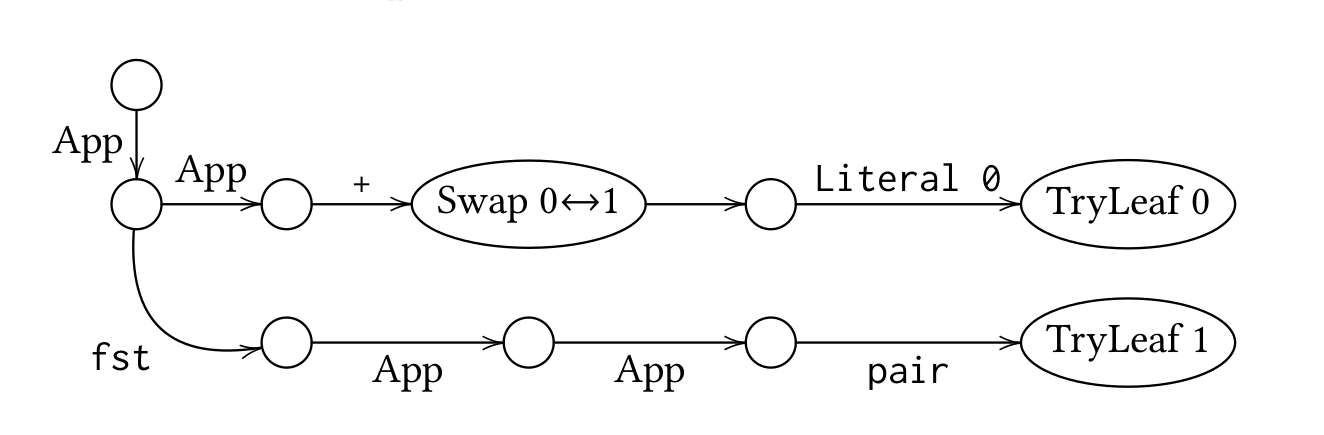
\includegraphics[width=\textwidth]{pictures/decisionTree.png}
\end{center}

\end{frame}

\begin{frame}[fragile]
  \transwipe[direction=90]
  \frametitle{Normalization by Evaluation}
\begin{columns}
  \begin{column}{0.4\textwidth}
    \[t ::= t \rightarrow t \mid b \]
  \end{column}
  \begin{column}{0.6\textwidth}
    \[e ::= \lambda v . e \mid e \ e \mid v \mid c \]
  \end{column}
\end{columns}

\begin{align*}
  NbE_t(t_1 \rightarrow t_2) &= NbE_t(t_1) \rightarrow NbE_t(t_2) \\
  NbE_t(b) &= expr(b)
\end{align*}

\begin{align*}
  reify_t &: NbE_t(t) \rightarrow expr(t) \\
  reify_{t_1 \rightarrow t_2}(f) &= \lambda v. reify_{t_2}(f(reflect_{t_1}(v))) \\
  reify_{b}(f) &= f
\end{align*}

\begin{align*}
  reflect_t &: expr(t) \rightarrow NbE_t(t) \\
  reflect_{t_1 \rightarrow t_2} &= \lambda x. reflect_{t_2}(e(reify_{t_1}(x))) \\
  reflect_b(e) &= e
\end{align*}
\end{frame}

\begin{frame}[fragile]
  \transwipe[direction=90]
  \frametitle{Normalization by Evaluation}
\begin{align*}
  reduce &: expr(t) \rightarrow NbE_t(t) \\
  reduce(\lambda v. e) &= \lambda x . reduce ([x / v] e) \\
  reduce(e_1 \ e_2) &= (reduce(e_1)) (reduce(e_2)) \\
  reduce(x) &= x \\
  reduce(c) &= reflect(c)
\end{align*}

\begin{align*}
  NbE &: expr(t) \rightarrow expr(t) \\
  NbE(e) &= reify(reduce(e))
\end{align*}
\end{frame}

\begin{frame}[fragile]
  \transwipe[direction=90]
  \frametitle{Применение правила переписывания}
\begin{align*}
  reflect_t &: expr(t) \rightarrow NbE_t(t) \\
  reflect_{t_1 \rightarrow t_2} &= \lambda x. reflect_{t_2}(e(reify_{t_1}(x))) \\
  reflect_b(e) &= \cancel{e} \ rewriteHead(e)
\end{align*}
\end{frame}

\begin{frame}[fragile]
  \transwipe[direction=90]
  \frametitle{Реализация: переменные}
\begin{center}
  Самое сложное --- следить за переменными
\end{center}
  \bigskip
\begin{center}
  Варианты представления термов с переменными:
\end{center}

\begin{itemize}
  \item Представление переменных строками
  \item Индексы де Брауна
  \item Higher-order abstract syntax
  \item \emph{Parametric higher-order abstract syntax}
\end{itemize}
\end{frame}

\begin{frame}[fragile]
  \transwipe[direction=90]
  \frametitle{Higher-order abstract syntax}
\begin{align*}
  term &: Type \\
  App  &: term \rightarrow term \rightarrow term \\
  Abs  &: (term \rightarrow term) \rightarrow term
\end{align*}

\begin{align*}
  id &= Abs (\lambda x . x ) \\
  diverge &= App (Abs (\lambda x . App \ x \ x)) (Abs (\lambda x . App \  x \ x))
\end{align*}
\end{frame}

\begin{frame}[fragile]
  \transwipe[direction=90]
  \frametitle{Parametric higher-order abstract syntax}
\begin{align*}
  term(V) &: Type \\
  Var    &: V \rightarrow term (V) \\
  App    &: term(V) \rightarrow term(V) \rightarrow term(V) \\
  Abs    &: (V \rightarrow term(V)) \rightarrow term(V)
\end{align*}

\begin{align*}
  id &= Abs (\lambda x . Var \ x )
\end{align*}

\[Term = \forall V : Type. term (V)\]

\end{frame}

\begin{frame}[fragile]
  \transwipe[direction=90]
  \frametitle{PHOAS: подсчет переменных}
\begin{align*}
numVars &: term(unit) \rightarrow \mathbb(N)  \\
numVars (Var \_) &= 1 \\
numVars (App \ e_1 \ e_2) &= numVars(e_1) + numVars(e_2) \\
numVars (Abs \ e) &= numVars (e ())
\end{align*}

\begin{align*}
NumVars &: Term \rightarrow \mathbb(N) \\
NumVars (E) &= numVars (E \ unit) \\
\end{align*}
\end{frame}

\begin{frame}[fragile]
  \transwipe[direction=90]
  \frametitle{PHOAS: допустимость $\eta$-редукции ($\lambda x. M \ x \rightarrow M$)}
\begin{align*}
canEta' &: term(bool) \rightarrow bool \\
canEta' (Var \ b) &= b \\
canEta' (App \ e_1 \ e_2) &= canEta'(e_1) \ \&\& \ canEta'(e_2) \\
canEta' (Abs \ e) &= canEta' (e \ true)
\end{align*}

\begin{align*}
  canEta &: term(bool) \rightarrow bool \\
  canEta (Abs e) &= match \ e \ false \ with \\
                 &\mid App \ e_1 (Var \ false) \Rightarrow canEta'(e_1) \\
                 &\mid \_ \Rightarrow false \\
  CanEta &: Term \rightarrow bool \\
  CanEta (E) &= canEta (E \ bool)
\end{align*}
\end{frame}

\begin{frame}[fragile]
  \transwipe[direction=90]
  \frametitle{PHOAS: capture-avoiding substitution}
\begin{align*}
subst &: \forall V : Type. term(term \ V) \rightarrow term(V) \\
subst (Var \ e) &= e \\
subst (App \ e_1 \ e_2) &= App (subst(e_1)) (subst(e_2)) \\
subst (Abs \ e) &= Abs (\lambda x. subst(e (Var \ x)))
\end{align*}

\begin{align*}
  Term1 &= \forall V : Type . \ V \rightarrow term(V) \\
  Subst &: Term1 \rightarrow Term \rightarrow Term \\
  Subst \ E_1 \ E_2 &= \forall V:Type . \ subst(E_1\ (term(V) \ (E_2\ V))
\end{align*}
\end{frame}

\begin{frame}[fragile]
  \transwipe[direction=90]
  \frametitle{PHOAS: представление целевого языка}
\begin{lstlisting}[basicstyle=\footnotesize]
Inductive type := arrow (s d : type)
| base (b : base_type).
Infix "->" := arrow.
Inductive expr (var : type -> Type) : type -> Type :=
| Var {t} (v : var t) : expr var t
| Abs {s d} (f : var s -> expr var d) : expr var (s -> d)
| App {s d} (f : expr var (s -> d)) (x : expr var s) :
expr var d
| Const {t} (c : const t) : expr var t
Definition Expr (t : type) : Type :=
  forall var, expr var t.
\end{lstlisting}
\end{frame}

\begin{frame}[fragile]
  \transwipe[direction=90]
  \frametitle{Дополнительные условия}
  \[n_1 + m - n_2 \rightarrow m, n_1 = n_2\]

  \begin{itemize}
    \item Условия --- вычислимые булевы функции на переменных, которые являются константами времени компиляции
    \item Реификация ожидает найти реализацию предиката среди гипотез
    \item Если в них используются переменные-не-константы, то применять правило переписывания нельзя
    \bigskip
    \item Некоторые ограничения можно получать из абстрактной интерпретации
  \end{itemize}
\end{frame}

\begin{frame}[fragile]
  \transwipe[direction=90]
  \frametitle{Эвалюация}

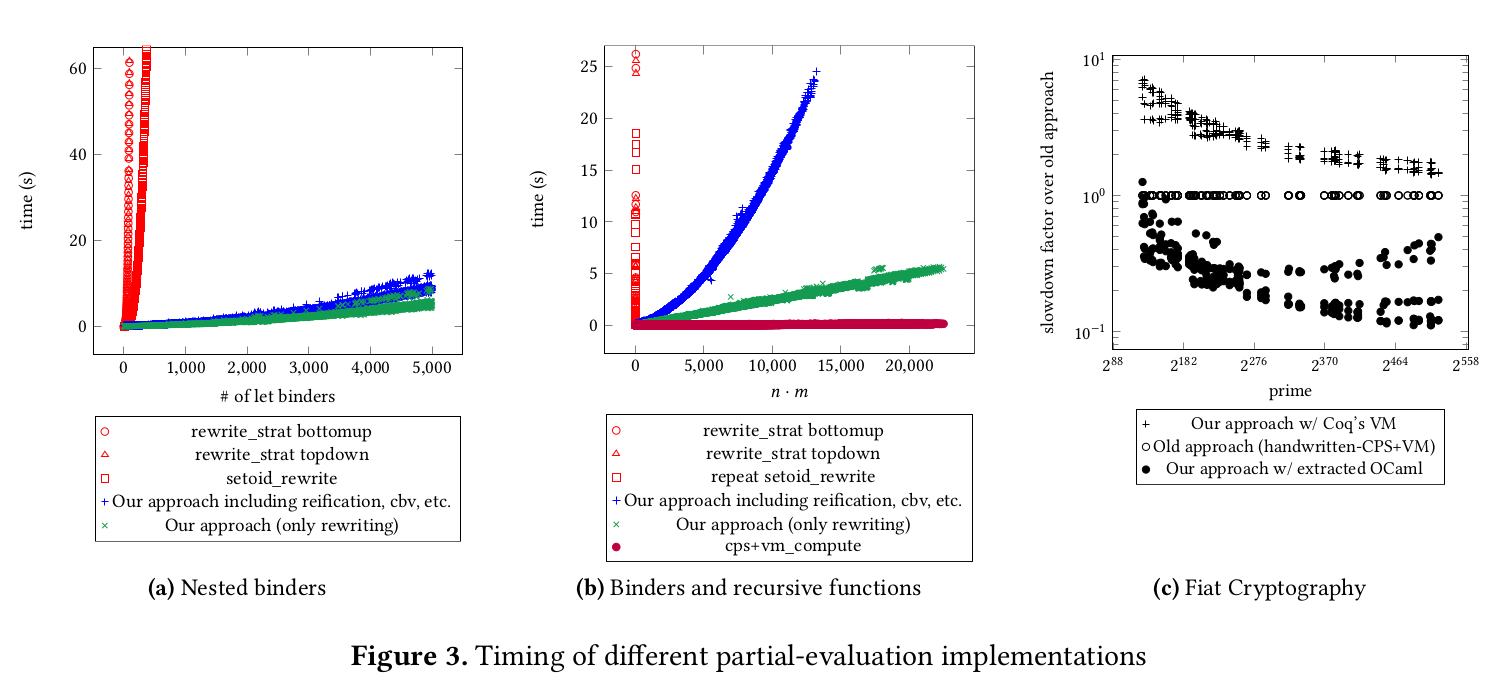
\includegraphics[width=\textwidth]{pictures/evaluation.png}
\end{frame}

\begin{frame}[fragile]
  \transwipe[direction=90]
  \frametitle{Источники}

  \begin{itemize}
    \item \href{https://people.csail.mit.edu/jgross/personal-website/papers/2020-rewriting-pldi-draft.pdf}{Jason Gross. A Framework for Building Verified Partial Evaluators}
    \begin{itemize}
      \item \href{https://github.com/mit-plv/rewriter}{Библиотека}
    \end{itemize}
    \item \href{https://citeseerx.ist.psu.edu/viewdoc/summary?doi=10.1.1.561.7972}{Klaus Aehlig et al. A compiled implementation of normalization by evaluation}
    \item \href{http://adam.chlipala.net/papers/PhoasICFP08/PhoasICFP08.pdf}{Adam Chlipala. Parametric Higher-Order Abstract Syntax for Mechanized Semantics}
  \end{itemize}

\end{frame}



\end{document}
